\documentclass[xcolor=dvipsnames,table,10pt]{beamer}
%\documentclass[xcolor=dvipsnames,table,10pt, aspectratio=169]{beamer}
\usepackage{newcent}
\usepackage{listings}
\usepackage[utf8]{inputenc}
\usepackage[czech]{babel}
\usepackage[T1]{fontenc}
\usepackage{hyperref}
\usepackage{fancyvrb}
\usepackage{subcaption}
\usetheme{FIT}

%%%%%%%%%%%%%%%%%%%%%%%%%%%%%%%%%%%%%%%%%%%%%%%%%%%%%%%%%%%%%%%%%%
\title[]{Nejv\v{e}t\v{s}\'i klika\\v neorientovan\'em grafu}

\author[]{Luk\'a\v{s} Lev}

%\institute[]{Brno University of Technology, Faculty of Information Technology\\
%Bo\v{z}et\v{e}chova 1/2, 612 00 Brno -- Kr\'alovo Pole\\
%login@fit.vutbr.cz}

\institute[]{Fakulta informa\v{c}n\'ich technologi\'i
Vysok\'eho u\v{c}en\'i technick\'eho v Brn\v{e}\\
Bo\v{z}et\v{e}chova 1/2, 612 00 Brno -- Kr\'alovo Pole\\
256660@vutbr.cz}

% \v{C}esk\'e logo - Czech logo
% beamerouterthemeFIT.sty \v{r}\'adek 9: fitlogo1_cz

%\date{January 1, 2024}
\date{\today}
%\date{} % bez data / without date

%%%%%%%%%%%%%%%%%%%%%%%%%%%%%%%%%%%%%%%%%%%%%%%%%%%%%%%%%%%%%%%%%%

\begin{document}

\frame[plain]{\titlepage}

\begin{frame}\frametitle{Zad\'an\'i}
    \textbf{Zad\'an\'i varianty}\\
    Vytvo\v{r}te program pro hled\'an\'i nejv\v{e}t\v{s}\'i kliky v neorientovan\'em grafu. Pokud existuje v\'ice \v{r}e\v{s}en\'i, \emph{nalezn\v{e}te v\v{s}echna}. V\'ysledky prezentujte vhodn\'ym zp\r{u}sobem. Sou\v{c}\'ast\'i projektu bude \emph{na\v{c}\'it\'an\'i graf\r{u}} ze souboru a vhodn\'e \emph{testovac\'i grafy}. V dokumentaci uve\v{d}te teoretickou slo\v{z}itost \'ulohy a \emph{porovnejte} ji s experiment\'aln\'imi v\'ysledky.\\[5pt]

    \textbf{\v{R}e\v{s}en\'i mus\'i obsahovat:}
    \begin{itemize}
        \item algoritmus pro nalezen\'i v\v{s}ech nejv\v{e}t\v{s}\'ich klik v neorientovan\'em grafu,
        \item na\v{c}\'it\'an\'i a zapisov\'an\'i graf\r{u} do souboru,
        \item testovac\'i grafy,
        \item porovn\'an\'i teoretick\'e slo\v{z}itosti s experiment\'aln\'imi v\'ysledky.
    \end{itemize}    
\end{frame}

\begin{frame}{Algoritmy a implementace}
    \textbf{Vybran\'e algoritmy:}
    \begin{itemize}
        \item hrub\'a s\'ila (\textit{brute force}),
        \item zp\v{e}tn\'e vyhled\'av\'an\'i (\textit{backtracking}).
    \end{itemize}
    \\[10pt]
    \textbf{Reprezentace neorientovan\'eho grafu} pomoc\'i matice sousednosti (kapitola 4.3)
    \begin{itemize}
        \item v\'yhody
        \begin{itemize}
            \item jednoduchost
        \end{itemize}
        \item nev\'yhody
        \begin{itemize}
            \item $O(n^2)$ prostorov\'e slo\v{z}itosti
            \item charakter \'ulohy $\implies$ iterace v\v{s}emi podgrafy $\implies$ $O(2^n)$
        \end{itemize}
    \end{itemize}
\end{frame}

\begin{frame}{Algoritmy a implementace}
    \begin{equation} \label{eq:adj-mat}
        \mathrm{M_s} = 
        \begin{pmatrix}
            h_{00} & h_{01} & h_{02} & h_{03} & h_{04} \\
            h_{10} & h_{11} & h_{12} & h_{13} & h_{14} \\
            h_{20} & h_{21} & h_{22} & h_{23} & h_{24} \\
            h_{30} & h_{31} & h_{32} & h_{33} & h_{34} \\
            h_{40} & h_{41} & h_{42} & h_{43} & h_{44}
        \end{pmatrix} = 
        \begin{pmatrix}
            0 & 0 & 0 & 1 & 1 \\
            0 & 0 & 1 & 0 & 1 \\
            0 & 1 & 0 & 1 & 0 \\
            1 & 0 & 1 & 0 & 1 \\
            1 & 1 & 0 & 1 & 0
        \end{pmatrix}
    \end{equation}
\end{frame}

\begin{frame}{Algoritmy a implementace}
    \begin{figure}
        \centering
        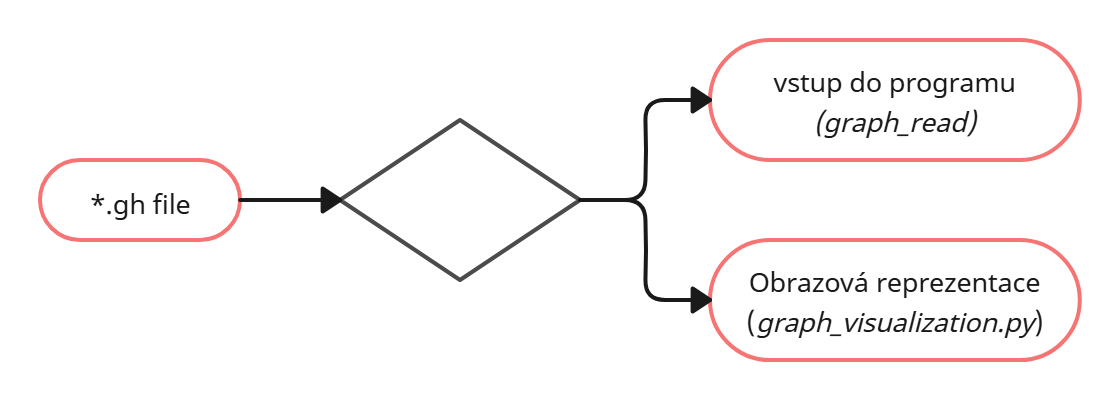
\includegraphics[width=0.7\linewidth]{dokumentace/pic/fc_1_gh.png}
    \end{figure}
    \begin{minipage}{.5\textwidth}
        \centering
        {\setmonofont{}\texttt{
5\\
0 0 0 1 1\\
0 0 1 0 1\\
0 1 0 1 0\\
1 0 1 0 1\\
1 1 0 1 0}}
    \end{minipage}%
    \begin{minipage}{.5\textwidth}
        \centering
        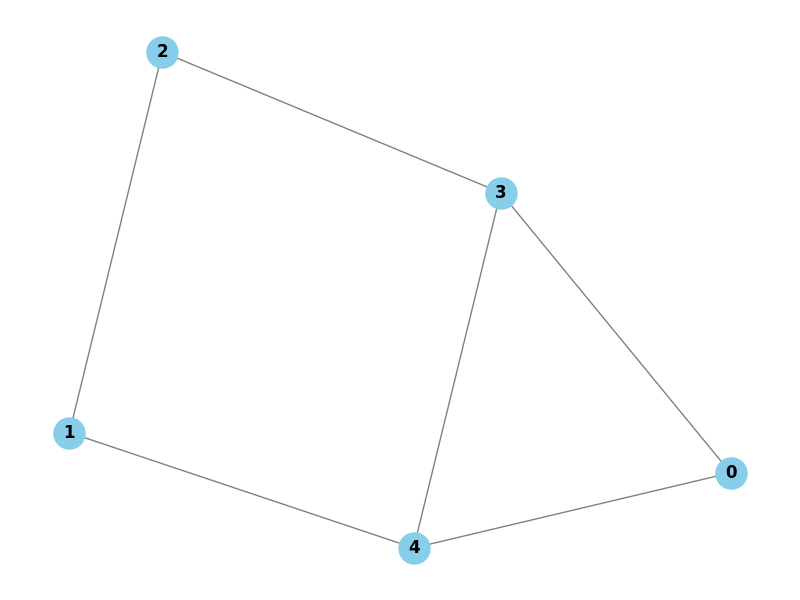
\includegraphics[width=\textwidth]{dokumentace/pic/graf_1.png}
    \end{minipage}
    
\end{frame}

\begin{frame}{Algoritmus metodou hrub\'e s\'ily}
    \begin{itemize}
        \item bitov\'a maska
        \begin{itemize}
            \item $10_{(10)} = 01010_{(2)} \implies u_{0}u_{1}u_{2}u_{3}u_{4}$\\[10pt]
        \end{itemize}
        \item \v{c}asov\'a slo\v{z}itost $\mathbf{O(2^n\cdot n^2)}$
        \begin{itemize}
            \item $2^n$ mo\v{z}n\'ych podgraf\r{u}
            \item nejh\r{u}\v{r}e kontrola $\binom{n}{2} = \frac{n(n-1)}{2} \implies n^2$ pro podgraf velikosti n\\[10pt]
        \end{itemize}
        \item prostorov\'a slo\v{z}itost $\mathbf{O(2^n\cdot n)}$
        \begin{itemize}
            \item pro $2^n$ cykl\r{u} ulo\v{z}eno $n$ prvk\r{u}
        \end{itemize}
    \end{itemize}
\end{frame}

\begin{frame}{Algoritmus metodou zp\v{e}tn\'eho vyhled\'av\'an\'i}
\begin{itemize}
        \item \v{c}asov\'a slo\v{z}itost $\mathbf{O(2^n\cdot n)}$
        \begin{itemize}
            \item $2^n$ mo\v{z}n\'ych podgraf\r{u}
            \item nejh\r{u}\v{r}e a\v{z} $n$ iterac\'i\\[10pt]
        \end{itemize}
        \item prostorov\'a slo\v{z}itost $\mathbf{O(2^n\cdot n)}$
        \begin{itemize}
            \item pro $2^n$ cykl\r{u} ulo\v{z}eno $n$ prvk\r{u}
        \end{itemize}
    \end{itemize}
    \hspace{15pt}
    \begin{figure}[h!]
        \centering
        \begin{subfigure}{0.3\textwidth}
            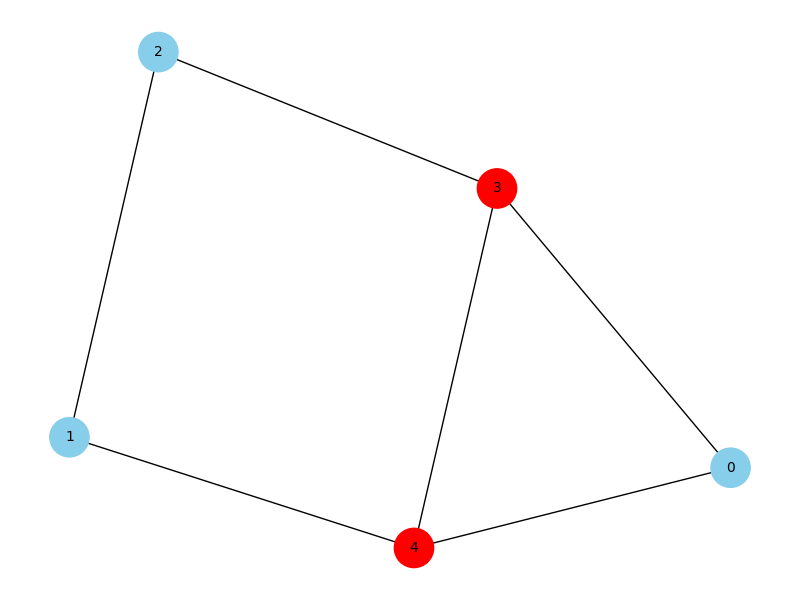
\includegraphics[width=\linewidth]{dokumentace/pic/graf_1_34.png}
        \end{subfigure}
        \hfill
        \begin{subfigure}{0.3\textwidth}
            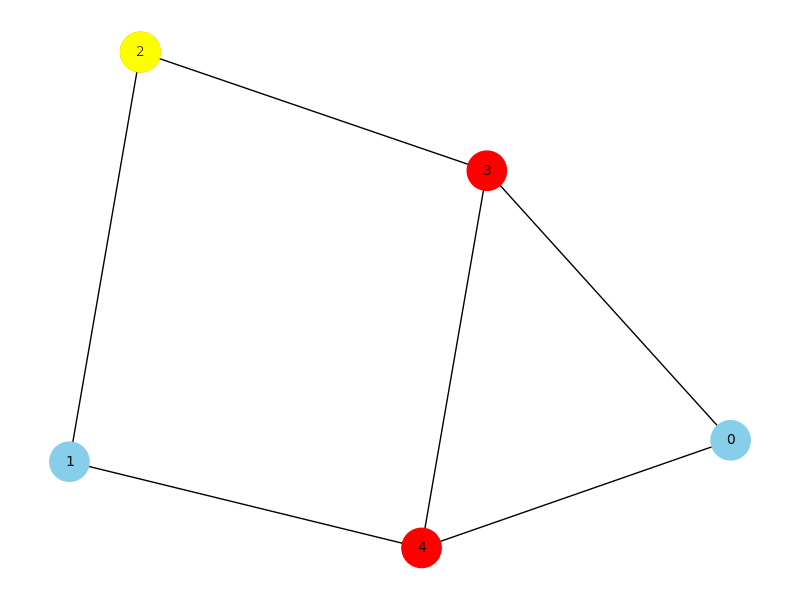
\includegraphics[width=\linewidth]{dokumentace/pic/graf_1_234_2.png}
        \end{subfigure}
        \hfill
        \begin{subfigure}{0.3\textwidth}
            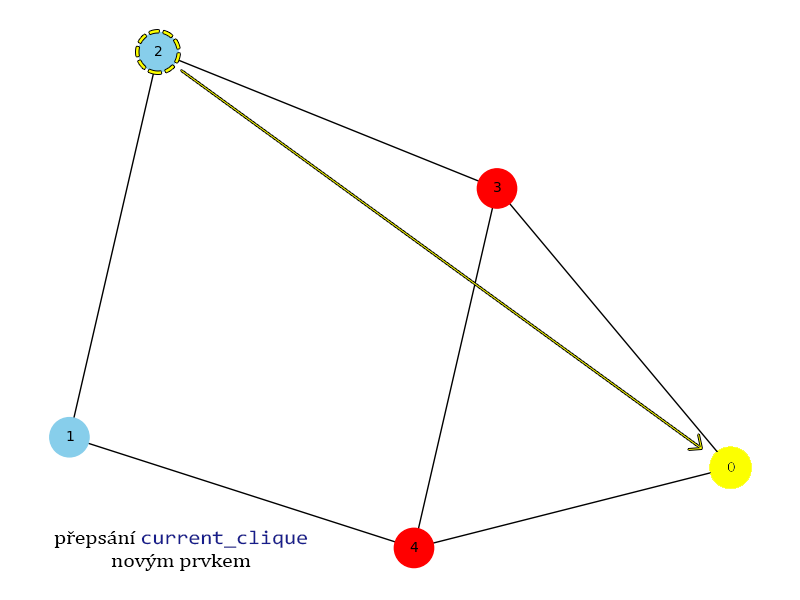
\includegraphics[width=\linewidth]{dokumentace/pic/graf_1_340.png}
        \end{subfigure}
    \end{figure}
    
\end{frame}


\begin{frame}{Experiment}
    \begin{enumerate}
        \item $\forall n \in \left<30;300\right> \cap \mathbb{N}$, $\rho = 0,5$, algoritmus metody zp\v{e}tn\'eho vyhled\'av\'an\'i\\[10pt]
        \item $\forall n \in \left<5;30\right> \cap \mathbb{N}$, $\rho = 0,5$, algoritmus metody hrub\'e s\'ily\\[10pt]
        \item $\forall n \in \left<5;59\right> \cap \mathbb{N}$, $\forall \rho \in \bigcup_{k=1}^{9}0,1\cdot k$, algoritmus metody zp\v{e}tn\'eho vyhled\'av\'an\'i\\[10pt]
        \item $\forall n \in \left<5;92\right> \cap \mathbb{N}$, $\forall \rho \in \bigcup_{k=1}^{9}0,1\cdot k$, algoritmus metody hrub\'e s\'ily
    \end{enumerate}    
\end{frame}

\begin{frame}{Experiment 1. a 2.}
    \textbf{Teoretick\'y p\v{r}edpoklad} (horn\'i hranice stanovena funkc\'i Omikron)
    \begin{figure}
        \centering
        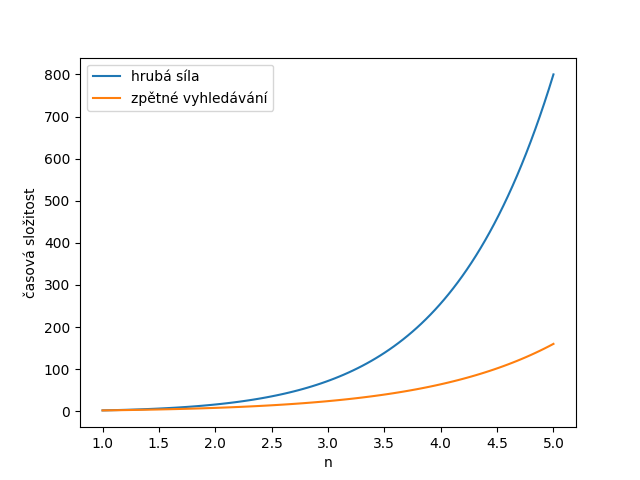
\includegraphics[width=.8\linewidth]{dokumentace/exp_vyhodnoceni/theo_lin_lin.png}
    \end{figure}
    
\end{frame}

\begin{frame}{Experiment 1. a 2.}
    \textbf{Teoretick\'y p\v{r}edpoklad} (funkce Omikron)\\
    logaritmick\'e \v{s}k\'alov\'an\'i
    \begin{figure}
        \centering
        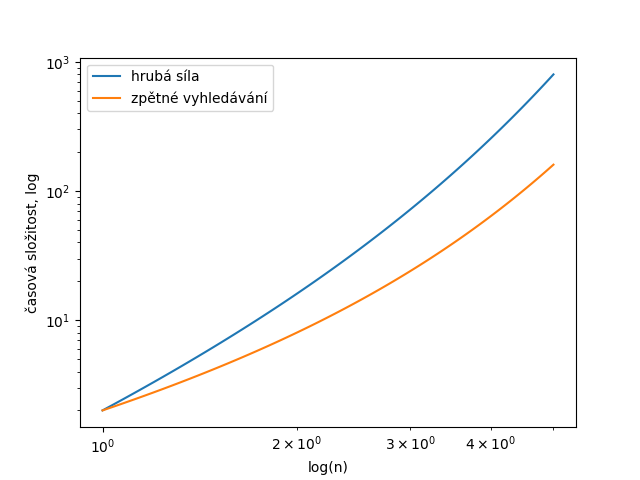
\includegraphics[width=.8\linewidth]{dokumentace/exp_vyhodnoceni/theo_log_log.png}
    \end{figure}
    
\end{frame}

\begin{frame}{Experiment 1. a 2.}
    \textbf{V\'ysledek experimentu}
    \begin{figure}
        \centering
        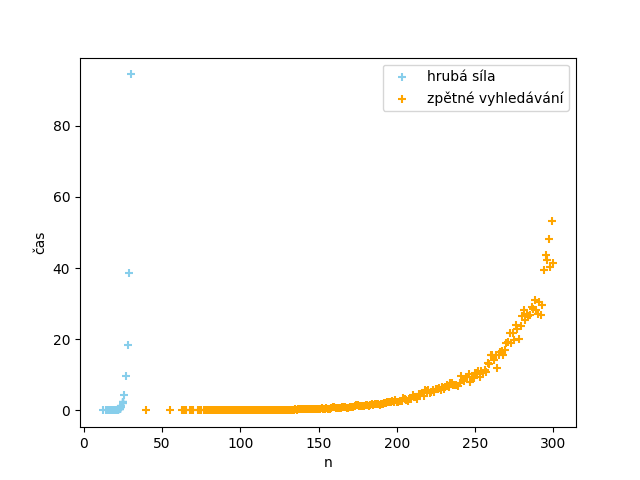
\includegraphics[width=.8\linewidth]{dokumentace/exp_vyhodnoceni/exp_lin_lin.png}
    \end{figure}
    
\end{frame}

\begin{frame}{Experiment 1. a 2.}
    \textbf{V\'ysledek experimentu}\\
    logaritmick\'e \v{s}k\'alov\'an\'i
    \begin{figure}
        \centering
        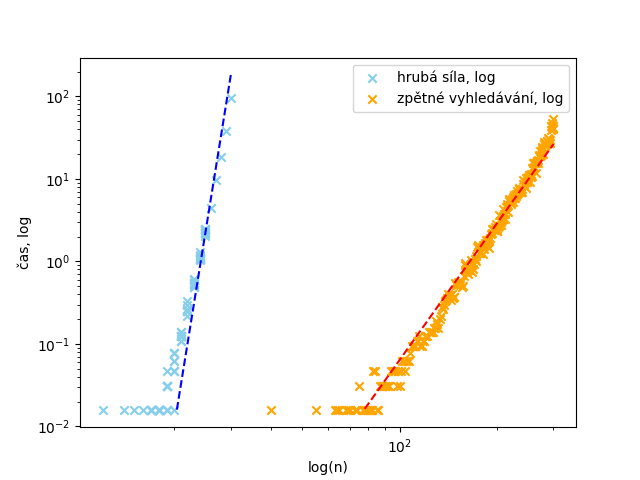
\includegraphics[width=.8\linewidth]{dokumentace/exp_vyhodnoceni/exp_log_log.png}
    \end{figure}
    
\end{frame}

\begin{frame}{Experiment 1. a 2.}
    \begin{figure}[h!]
        \centering
        \begin{subfigure}{0.49\textwidth}
            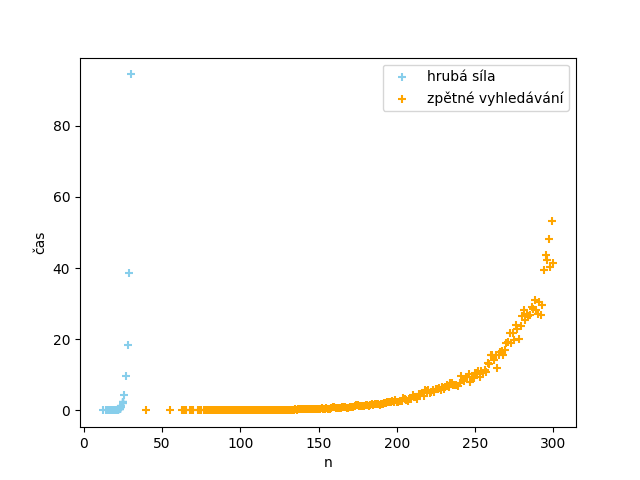
\includegraphics[width=\linewidth]{dokumentace/exp_vyhodnoceni/exp_lin_lin.png}
        \end{subfigure}
        \hfill
        \begin{subfigure}{0.49\textwidth}
            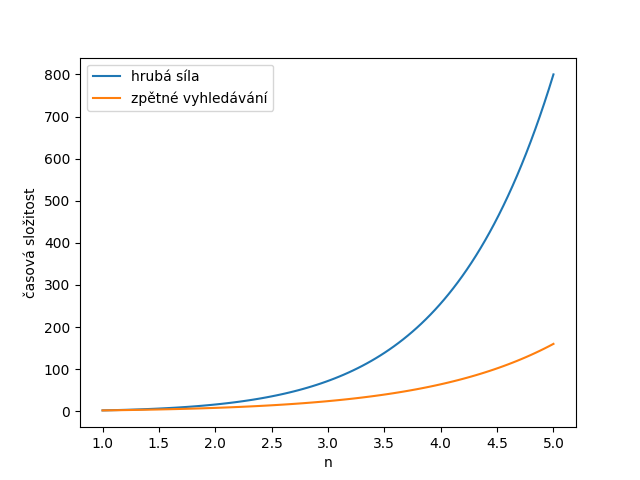
\includegraphics[width=\linewidth]{dokumentace/exp_vyhodnoceni/theo_lin_lin.png}
        \end{subfigure}
    \end{figure}
\end{frame}
\begin{frame}{Experiment 1. a 2.}
    \begin{figure}[h!]
        \centering
        \begin{subfigure}{0.49\textwidth}
            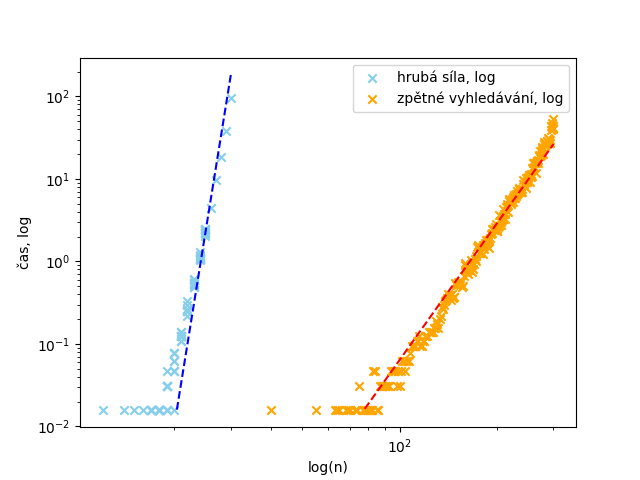
\includegraphics[width=\linewidth]{dokumentace/exp_vyhodnoceni/exp_log_log.png}
        \end{subfigure}
        \hfill
        \begin{subfigure}{0.49\textwidth}
            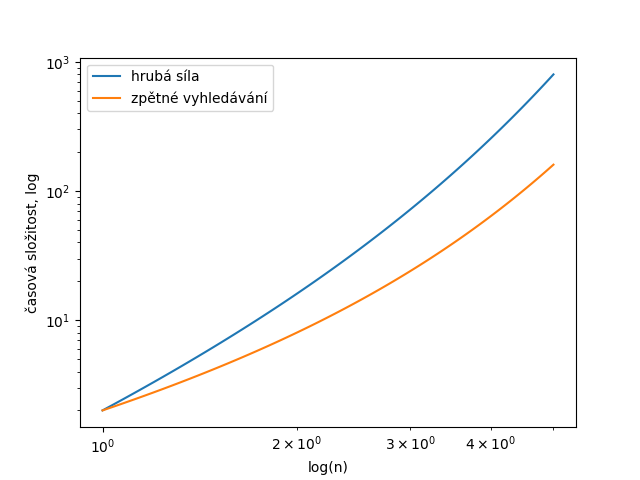
\includegraphics[width=\linewidth]{dokumentace/exp_vyhodnoceni/theo_log_log.png}
        \end{subfigure}
    \end{figure}
\end{frame}

\begin{frame}{Experiment 3. a 4.}
    \textbf{V\'ysledek experimentu}
    \begin{figure}
        \centering
        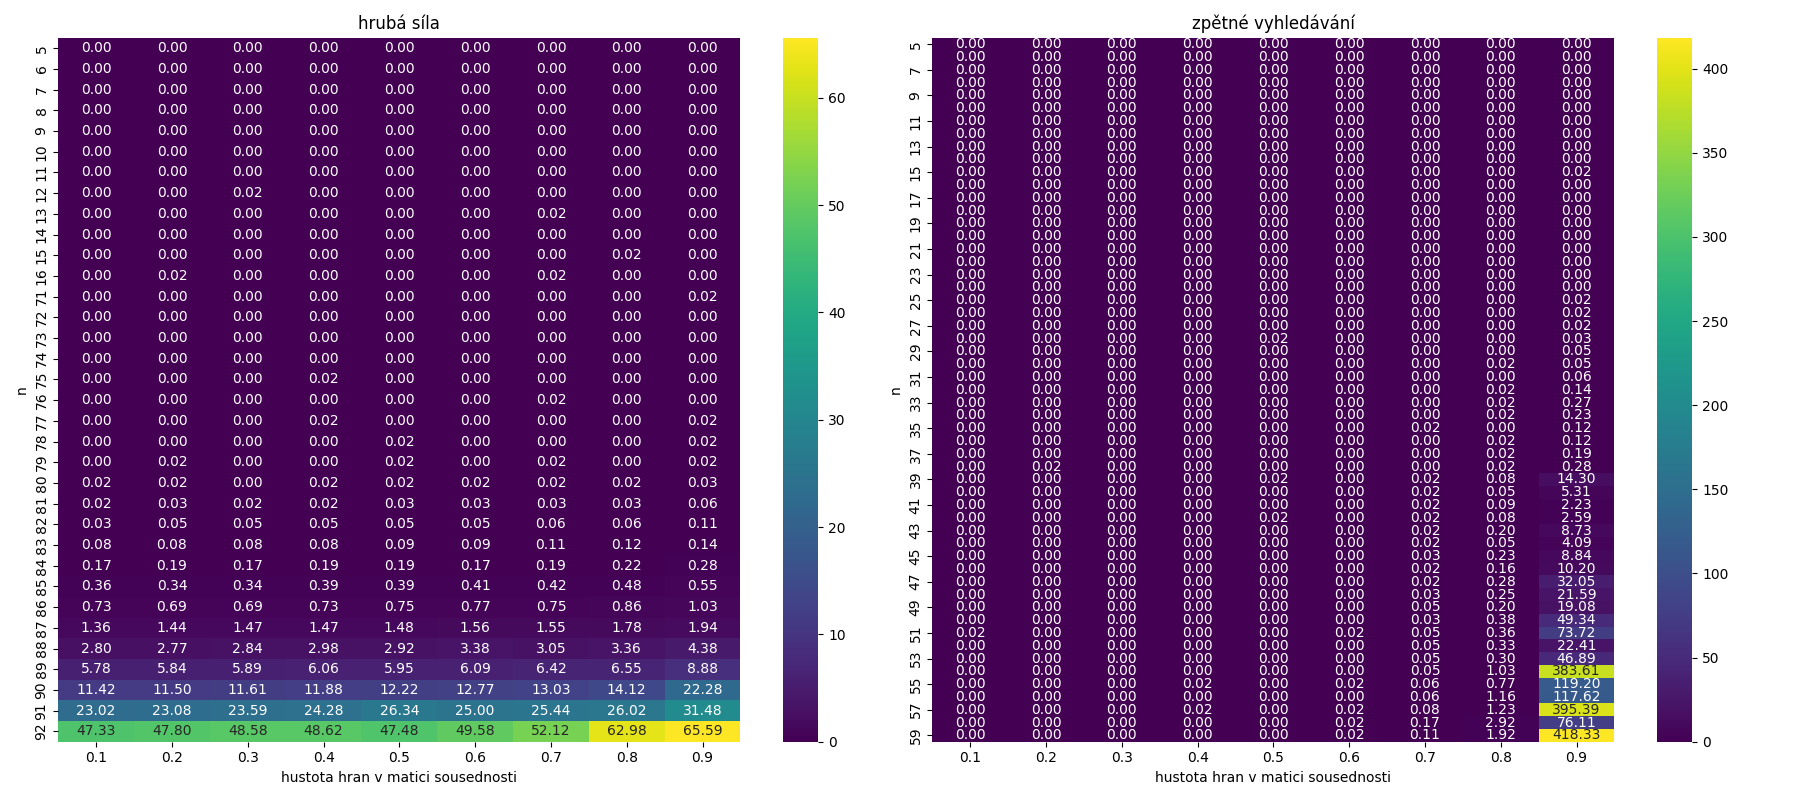
\includegraphics[width=\linewidth]{dokumentace/exp_vyhodnoceni/n_dens.png}
    \end{figure}
    
\end{frame}

\begin{frame}{Experiment 3. a 4.}
    \textbf{V\'ysledek experimentu}\\
    logaritmick\'e \v{s}k\'alov\'an\'i
    \begin{figure}
        \centering
        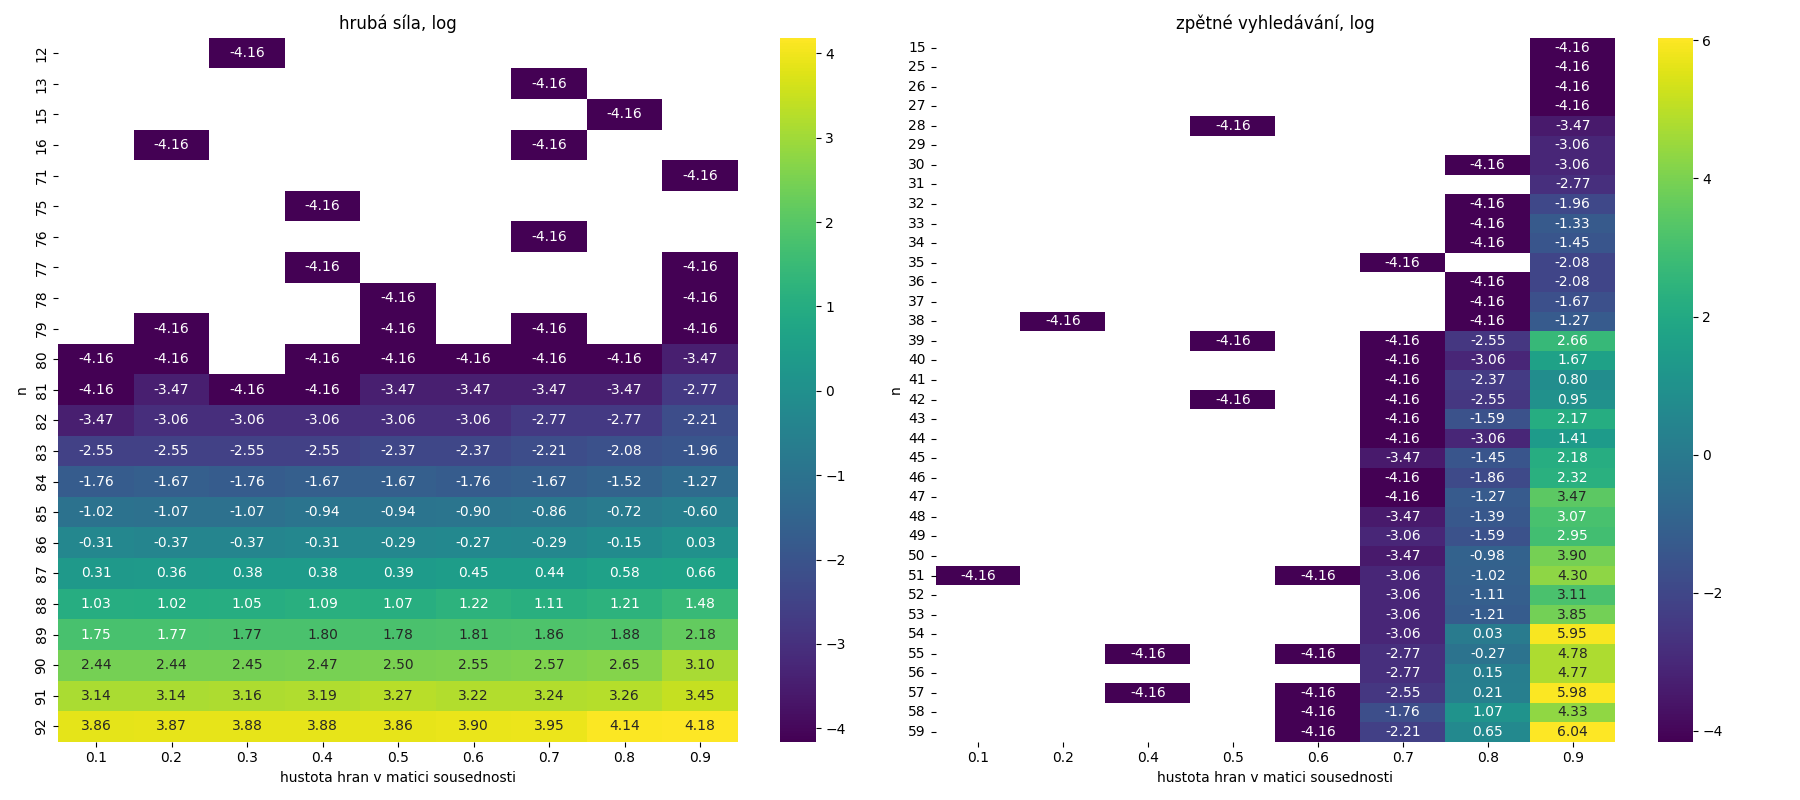
\includegraphics[width=\linewidth]{dokumentace/exp_vyhodnoceni/log_n_dens.png}
    \end{figure}
    
\end{frame}

\begin{frame}{Z\'av\v{e}r}
    \begin{itemize}
        \item porovn\'an\'i teoretick\'ych p\v{r}edpoklad\r{u} \v{c}asov\'e slo\v{z}itosti s experimentem\\[15pt]
        \item ur\v{c}en\'i vhodn\'e aplikace pro ka\v{z}d\'y z algoritm\r{u}\\[15pt]
        \item nast\'in\v{e}n\'i dal\v{s}\'ich krok\r{u} pro p\v{r}esn\v{e}j\v{s}\'i porovn\'an\'i teorie s experimentem
    \end{itemize}
\end{frame}


\bluepage{D\v{e}kuji za pozornost.}

\end{document}
